% RULE APPEARANCE:
\newcommand{\x}{\hspace{1.3pt}} % arithmetic multiplication symbol
\newcommand{\concat}[0]{\bullet}               % list concatenation symbol
\newcommand{\name}[1]{~~\hfill\framebox{#1}}   % for labeling rules

% RULE SPACING:
\newcommand{\skiptop}[0]{\vspace{-13pt}\\}   % for single line on top
\newcommand{\skiptopa}[0]{\vspace{-1pt}\\}   % for first line of two-line top part
\newcommand{\skiptopb}[0]{\vspace{-3pt}\\}   % for second line of two-line top part
\newcommand{\skipbot}[0]{\vspace{-3pt}\\}    % for single line on botto

% HELPER FOR REPEATS:
\newcommand{\tup}[2]{\langle#1, #2\rangle}

% OUR LABEL FOR THE ``POS'' VARIABLE
\newcommand{\pos}[0]{\mbox{\it pos}}

% MY TAB STOP FOR THE PSEUDOCODE
\newcommand{\tab}[0]{\mbox{~~~~}}

%%%%%%%%%%%%%%%%%%%%%%%%%%%%%%%%%%%%%%%%%%%%%%%%%%%%%%%%%%%%%%%%%%%%%%%%%%

\section{Program Representation}

Our transformation relies on the cyclo-static dataflow representation
for input programs and the LZ77 representation of compressed data.
These are described in the next two sections.

\subsection{Cyclo-Static Dataflow}

In the cyclo-static dataflow model, a program is represented by a set
of independent {\it actors} that communicate using FIFO data
channels~\cite{LM87-i,bilsen95-cyclostatic}.  Each actor has an
independent program counter and address space; all communication is
done using the data channels.  Actors have one or more atomic
execution steps that execute in a fixed pattern throughout the
lifetime of the program.  A key restriction of the cyclo-static
dataflow model is that, for each execution of a given actor, the
number of items produced and consumed on the data channels is known at
compile time.  This enables the compiler to perform static scheduling
of the actors and to guarantee deadlock freedom~\cite{LM87-i,bilsen95-cyclostatic}.

Cyclo-static dataflow is a natural fit for many multimedia and signal
processing kernels, as such programs often have a regular structure
with known communication patterns.  As a programmer, one can use a
high-level language such as StreamIt~\cite{streamitcc} to express a
cyclo-static dataflow program.  An example StreamIt program appears in
Figure~\ref{fig:streamit}.  It reads lines of an RGB image from a
file, shrinks the image by a factor of two, inverts the color of each
pixel, then writes the data to a file.  There are three kinds of
actors in StreamIt programs, and our analysis handles each one
separately:
\begin{itemize}

\item {\bf Filters} have a single input stream and a single output
  stream, and perform general-purpose computation.  Filters perform
  the same function on every execution (there is no cyclic pattern of
  computations).  For example, in the {\tt InvertColor} filter, the
  {\tt work} function specifies the atomic execution step; it declares
  that on each execution, it pops (inputs) 1 item from the input tape
  and pushes (outputs) 1 item to the output tape.  Though StreamIt
  also allows filters to peek at the input stream (i.e., to perform a
  sliding window computation) and to maintain mutable state across
  executions, these features are uncommon in other stream languages
  and we do not support them in the current work.

\item {\bf Splitters} have a single input stream and multiple output
  streams, and perform pre-defined computations.  There are two types
  of splitters: {\it duplicate} splitters, which replicate their
  inputs to all of the target streams, and {\it roundrobin} splitters,
  which distribute the input items across the streams.  Roundrobin
  splitters are parameterized: roundrobin$(n_1, n_2)$ indicates that
  the first $n_1$ items are sent to the first output, and the next
  $n_2$ items are sent to the second output.  Splitters execute in a
  fine-grained, cyclo-static fashion; regardless of the parameters,
  each execution step passes only a single item from the input stream
  to an output stream.  In Figure~\ref{fig:streamit}, the splitter
  sends {\tt WIDTH} pixels in each direction, serving to distribute
  lines of the image across different streams.

\begin{figure}[t]
\psfig{figure=streamit-figure.eps,width=3.408in}
\caption{Example StreamIt program.
\protect\label{fig:streamit}}
\end{figure}

\item {\bf Joiners} have multiple input streams and a single output
  stream, and perform pre-defined computations.  The only type of
  joiner is roundrobin, which acts analogously to a roundrobin
  splitter.  In Figure~\ref{fig:streamit}, the joiner reads one pixel
  at a time from each input stream, serving to interleave the pixels
  from neighboring lines.  Once the pixels are interleaved, each group
  of 4 pixels is averaged together in order to decrease the picture
  width by two.

\end{itemize}

\subsection{LZ77 Compression}

LZ77 is a lossless, dictionary-based compression algorithm.  Named
after its creators Lempel and Ziv, who published the algorithm in
1977~\cite{lz77}, LZ77 is asymptotically optimal~\cite{wyner94optimal}
and forms the basis for many popular compression formats, including
ZIP, GZIP and PNG.  As described in Section~\ref{sec:formats}, LZ77
also serves as a generalization of simpler encodings such as Apple
Animation, Microsoft RLE, and Targa, allowing our transformations to
naturally extend to these formats.

\begin{figure}[t]
\begin{minipage}{1.6in}
\hspace{-5pt}\begin{tabular}{rcl}
stream&\hspace{-9pt}:=&\hspace{-9pt}value$^*$\\ ~ & ~
\end{tabular}
\end{minipage}
\begin{minipage}{1.8in}
\hspace{-5pt}\begin{tabular}{rcl}
stream&\hspace{-9pt}:=&\hspace{-9pt}(value~$|$~repeat)$^*$ ~ \\
repeat&\hspace{-9pt}:=&\hspace{-9pt}$\langle$distance, count$\rangle$
\end{tabular}
\end{minipage} 
~ \\
\begin{minipage}{1.6in}
(a) Uncompressed domain
\end{minipage}
(b) Compressed domain (LZ77)
\caption{Representation of data in the uncompressed and compressed
domains.  \protect\label{fig:domains}}
\end{figure}

The basic idea behind LZ77 is to utilize a sliding window of recently
encoded values as the dictionary for the compression algorithm.  In
the compressed data stream, there are two types of tokens: {\it
values} and {\it repeats} (see Figure~\ref{fig:domains}).  A value
indicates a token that should be copied directly to output of the
decoded stream.  A repeat contains two parts: a distance $d$ and a
count $c$; it indicates that the decoder should start at offset $d$
from the end of the decoded stream and copy a sequence of $c$ values
to the output.  The distances are bounded, which enables the decoder
to operate with a fixed buffer size.  It is important to note that the
count may exceed the distance, in which case some of the values
produced by a repeat operation are also copied by that operation.  For
example, a value A followed by a repeat $\tup{1}{3}$ results in an
output of ``A A A''.  An additional example of LZ77 decoding is given
in Figure~\ref{fig:lz77}.

\begin{figure}[t]
\begin{minipage}{0.21in}
\mbox{~}
\end{minipage}
\psfig{figure=lz77-figure.eps,width=2.6in}
\caption{Example of LZ77 decompression.
\protect\label{fig:lz77}}
\end{figure}

\newcommand{\tablesep}{\hspace{-3.5pt}}
\begin{figure}[t]
\hspace{-5pt}\begin{tabular}{llll}
\multicolumn{2}{l}{Variables} & \multicolumn{2}{l}{{\tablesep}Constants} \\ \rule[10pt]{1.9in}{0.3pt}\hspace{0.1in}\rule[10pt]{1.3in}{0.3pt}\hspace{-1.3in}\hspace{-2pt}\hspace{-1.97in}\hspace{-2pt}
$S$, $T$ & {\tablesep}Input, output streams & {\tablesep}$n_1$, $n_2$ & {\tablesep}Actor's pop rates \\
$V$ & {\tablesep}List of values (may be empty) & {\tablesep}$m$ & {\tablesep}Actor's push rate \\
$\tup{d}{c}$ & {\tablesep}Repeat distance \& count & {\tablesep}~ & ~ \vspace{6pt} \\
\multicolumn{2}{l}{Functions (list $\times$ list $\rightarrow$ list)}& ~ & ~ \\ \rule[10pt]{3.3in}{0.3pt}\hspace{-3.3in}
$\concat$ & {\tablesep}List concatenation & ~ & ~ \\
$F$ & \multicolumn{3}{l}{{\tablesep}Filter work function, outputs $m$-element list}
\end{tabular}
\caption{Notations used in the semantic rules.\protect\label{fig:notations}}
\end{figure}

\section{Program Transformation}
Our program transformation inputs a cyclo-static dataflow program and
outputs an equivalent program in which all of the data channels use a
compressed representation.  One can think of this process as mapping
from the uncompressed domain to the compressed domain (see
Figure~\ref{fig:domains}).  Rather than modifying the code within the
actors, our transformation treats actors as black boxes and wraps them
in a new execution layer.  The transformation attempts to preserve as
much compression as possible without ever performing an explicit
re-compression step.  While there exist cases in which the output data
will not be as compressed as possible, under certain conditions the
output is guaranteed to be fully compressed (relative to the
compression of the input).

For the sake of presentation, we use an operational semantics to
express the execution under the uncompressed and compressed domains.
Though some of the transition rules require dynamic data rates and
thus fall outside the cyclo-static dataflow model, all of them have an
efficient implementation in StreamIt.  The rules use the notations
given in Figure~\ref{fig:notations}, and have the following form:

\hspace{-12pt}\begin{tabular}{l} ~ \vspace{-6pt} \\ 
\hspace{-3pt}$S \rightarrow T$ \hspace{-7pt}~\vspace{0.5pt} \\ \hline ~ \vspace{-7.5pt} \\
\hspace{-3pt}$S' \rightarrow T'$ \hspace{-7pt} \\ ~ \vspace{-6pt} \\
\end{tabular}

This rule reads: if the incoming stream has value $S$ and the outgoing
stream has value $T$, then after an execution step, the streams have
values $S'$ and $T'$, respectively.  As detailed in
Figure~\ref{fig:domains}, we represent streams as lists of tokens;
inputs to the stream are added to the front of the list, while outputs
from the stream are removed from the end of the list.

To describe the mapping into the compressed domain, we consider
filters, splitters, and joiners in turn.

\subsection{Filters}

\begin{figure}[t]
$S \concat V \rightarrow T~~~~|V|=n$\name{exec-uncompressed} \skiptopb
---------------------------- \skipbot
$S \rightarrow F(V) \concat T$
\caption{Semantics of \textsc{Exec(F)}: execution of filter F in the
uncompressed domain.  Notations are defined in Figure~\ref{fig:notations}.
\protect\label{fig:exec-rule}}
\end{figure}

\begin{figure}[t]
~~~~~~~~~\psfig{figure=actor-figure.eps,width=2.8in}

\mbox{~}(a) Uncompressed domain~~~~~~~~~~~~~~~~~(b) Compressed domain
\caption{Overall execution of a filter F in the uncompressed and compressed domains.
\protect\label{fig:actor-pic}}
\end{figure}

Filter execution in the uncompressed domain is described by the rule
in Figure~\ref{fig:exec-rule}.  The rule expresses the simple fact
that a filter inputs a list of $n$ values from the end of its input
stream; this list is denoted by $V$.  The filter pushes its results,
denoted by $F(V)$, onto the front of the output stream.

Filter execution in the compressed domain requires a two-stage
transformation (see Figure~\ref{fig:actor-pic} for an overview, and
Figure~\ref{fig:filter-example} for a detailed example).  First, the
input stream is aligned to a granularity $n$ that matches the input
rate of the filter.  This alignment guarantees that every token in the
stream is either a sequence of $n$ values, or a repeat in which both
the distance and the count are multiples of $n$.  The alignment stage
is a no-op for filters that pop only one item ($n=1$).  It is
described in more detail below.

After the alignment stage comes the execution of the compressed
filter, which appears in Figure~\ref{fig:compressed-exec-rule}.  The
{\tt exec-uncompressed} rule
%(not shown in Figure~\ref{fig:compressed-exec-rule}) 
deals with values on the input stream, and is identical to that in the
uncompressed execution.  The {\tt exec-compressed} rule deals with
repeats on the input stream and encapsulates the key idea of the
paper.  Because the inputs are repeating at the correct granularity,
the repeat can be copied directly to the output of the filter without
performing any new computation.  The only change needed is to adjust
the repeat distance and count to match the filter's output rate.

\begin{figure*}[t]
\vspace{-6pt}
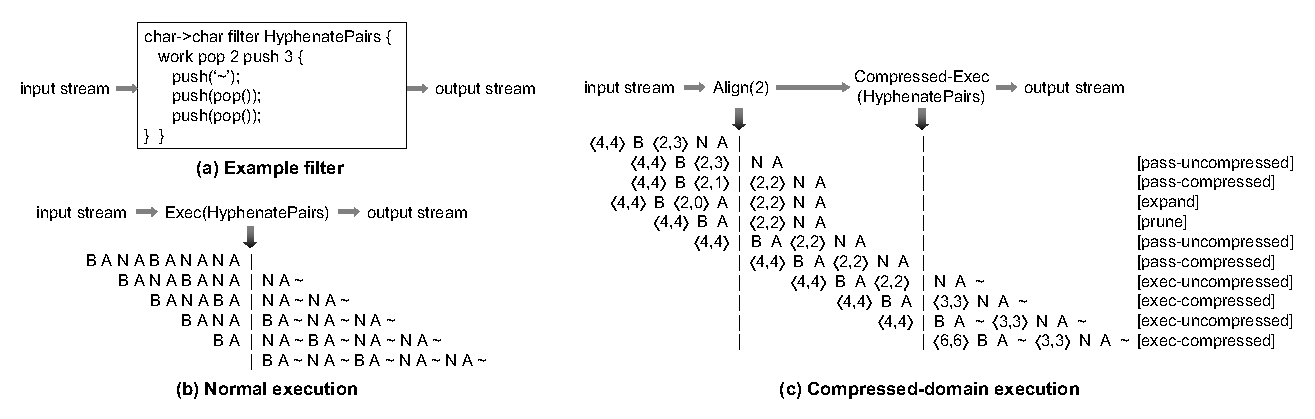
\psfig{file=compressed-filter-example.eps,width=\textwidth}
\vspace{6pt}
\caption{Example execution of a filter in the uncompressed and
  compressed domains.\protect\label{fig:filter-example}}
\end{figure*}

\begin{figure}[t]
$S \concat V \rightarrow T~~~~|V|=n$\name{exec-uncompressed} \skiptopb
---------------------------- \skipbot
$S \rightarrow F(V) \concat T$
~ \\ ~ \\
%\hfill\mbox{\it Same as above.}\name{exec-uncompressed}\vspace{6pt}\\
$S \concat \tup{d}{c} \rightarrow T~~~~d$\%$n=0~~~~c$\%$n=0$\name{exec-compressed} \skiptopb
------------------------------------------------ \skipbot
$S \rightarrow \tup{m{\x}d/n}{m{\x}c/n} \concat T$
\caption{Semantics of \textsc{Compressed-Exec(F)}: execution of filter
$F$ in the compressed domain.
%This filter also includes an {\tt exec-uncompressed} rule, which is
%identical to the one in Figure~\ref{fig:exec-rule}.
Notations are defined in Figure~\ref{fig:notations}.
\protect\label{fig:compressed-exec-rule}}
\end{figure}

\subsubsection{Stream Alignment}

The alignment phase is needed for filters that pop more than one item
from the input stream.  Its goal is to align the execution boundaries
of the filter with the repeat boundaries of the compressed data; this
alignment is required for the compressed execution.  Following
alignment, each execution of a filter will input either $n$
consecutive values, or a repeat token with a distance and count that
are evenly divisible by $n$ (where $n$ represents the pop rate of the
filter).

The alignment stage sometimes needs to partially decompress the data
in the stream.  Due to the sliding-window dictionary in LZ77, it is
difficult to decode only a few items without decompressing others.
Thus, our formulation assumes that a fully decompressed version of the
stream is available; the transition rules access the decompressed data
using the \mbox{\it decode} function, which returns the sequence of
values represented by a repeat token at its current position in the
stream.  However, as detailed in Section~\ref{sec:opt}, there are
important cases in which decompression can be completely avoided.
Even where decompression is needed, the overhead is minimal compared
to the costs of re-compression (which remains unnecessary because only
some of the decompressed data is injected into the stream).

The semantics of stream alignment are given in
Figure~\ref{fig:stream-align}.  If the end of the input stream
contains $n$ values, then alignment is satisfied and the values are
moved to the output stream (rule {\tt pass-uncompressed}).  Likewise,
if the input contains a repeat in which the distance is a multiple of
$n$ and the count is at least $n$, then a number of aligned repeats
are peeled from the input and moved to the output (rule {\tt
  pass-compressed}).  If the count is not a multiple of $n$, then part
of the repeat is leftover and remains on the input stream.

There are some cases in which a repeat cannot be moved to the output
stream, in which case the data needs to be partially decompressed
(rule {\tt expand}).  This occurs if the repeat has a count less than
$n$, if it occurs in the middle of an aligned stretch of $n$ values,
or if its distance is not a multiple of $n$ (this last condition can
sometimes be remedied by another rule, see below).  The {\tt expand}
rule decodes only one value from an unaligned repeat token, thereby
decreasing its count by one; the rest of the repeat may become aligned
later.  If the count of a repeat reaches zero, it is eliminated by the
{\tt prune} rule.

\begin{figure}[t]
$S \concat V \rightarrow T~~~|V|=n$\name{pass-uncompressed}\skiptopb
---------------------------\skipbot
$S \rightarrow V \concat T$
~ \\ ~ \\
$S \concat \tup{d}{c} \rightarrow T~~~d$\%$n=0~~~c \ge n$\name{pass-compressed}\skiptopb
------------------------------------------\skipbot
$S \concat \tup{d}{c$\%$n} \rightarrow \tup{d}{c-c$\%$n} \concat T$
~ \\ ~ \\
$S \concat \tup{d}{c} \concat V \rightarrow T~~~~~c\le\mbox{LCM}(d,n)$\name{expand}\\
$(c<n~\vee~1 \le |V|<n~\vee~d$\%$n>0)$\skiptopb
--------------------------------------------------\skipbot
$S \concat \tup{d}{c-1} \concat \mbox{\it decode}(\tup{d}{1}) \concat V \rightarrow T$
~ \\ ~ \\
$S \concat \tup{d}{0} \concat V \rightarrow T$\name{prune}\skiptopb
------------------------\skipbot
$S \concat V \rightarrow T$
~ \\ ~ \\
let~$L=\mbox{LCM}(d,n)$\name{coarsen-repeat}\\
$S \concat \tup{d}{c} \concat V \rightarrow T~~~~d$\%$n > 0~~~~c > L$\vspace{-3pt}\skiptopa
------------------------------------------------------\skipbot
$S \concat \tup{L}{c-(L-d)} \concat \tup{d}{L-d} \concat V \rightarrow T$
\caption{Semantics of \textsc{Align}($n$): aligning data
to a granularity of $n$.  The \mbox{\it decode} function uncompresses
a repeat token into a list of values; other notations are given in
Figure~\ref{fig:notations}. \protect\label{fig:stream-align}}
\end{figure}

The final rule, {\tt coarsen-repeat}, preserves a specific kind of
compression in the input stream.  Consider that a filter pops two
items at a time, but encounters a long repeat with distance three and
count 100.  That is, the input stream contains a regular pattern of
values with periodicity three.  Though consecutive executions of the
filter are aligned at different offsets in this pattern, every third
filter execution (spanning six values) falls at the same alignment.
In general, a repeat with distance $d$ can be exploited by a filter
with pop rate $n$ by expanding the distance to $\mbox{LCM}(d, n)$.  In
order to perform this expansion, the count must be greater than the
distance, as otherwise the repeat references old data that may have no
periodicity.  Also, the stream needs to be padded with $\mbox{LCM}-d$
values before the coarsened repeat can begin; this padding takes the
form of a shorter repeat using the original distance.

\subsubsection{Optimizations}
\label{sec:opt}

As the transformation to the compressed domain is formulated in
fully general terms, the process can be streamlined considerably for
common classes of inputs:
\begin{itemize}
\item If a filter has a pop rate of one ($n=1$) on a given stream then
  no alignment stage is needed.
\item If the repeat distance is equal to the LZ77 window size, then no
  decompression is needed because it would simply overwrite the same
  values in the buffer.  This property holds for inter-frame repeats
  in the Apple Animation format (see Section~\ref{sec:formats}).
\end{itemize}
A consequence of the first bullet is that filters with a pop rate of
one (such as the InvertColor filter in Figure~\ref{fig:streamit}) avoid
performing any decompression, as there is no alignment stage.  This
guarantees that the output of the filter will be the same size as the
compressed input.

%% \subsection{Extensions}
%% \label{sec:extensions}

%% The transformation can be extended to support a broader class of
%% filters.  Some straightforward extensions are as follows:
%% \begin{itemize}

%% \item {\it Filters with state.}  If a filter retains mutable state from
%% one execution to the next, a repeat token can be copied across the
%% filter if the current state values are the same as they were at the
%% beginning of the repeated segment.  One could maintain a lookup table
%% that tracks the state values for the sake of this comparison.  Also,
%% state updates that have a closed form can be applied in the compressed
%% domain even if the current state has never been seen before; for
%% example, if a histogram filter runs for $n$ iterations on a blue
%% pixel, it will increment the blue count by $n$ regardless of the
%% initial value.

%% \item {\it Dynamic input and output rates.}  The current formulation
%% relies on a filter's fixed I/O rates to calculate repeat distances and
%% counts for the output tape from the repeat tokens on the input tapes.
%% However, in the presence of unpredictable I/O rates (e.g., edge
%% detection), a lookup table could be used to track the actual I/O rates
%% on each execution.  In the event of a repeat, the recorded I/O rates
%% from the previous execution could be used to calculate the repeat
%% parameters on the output tape.

%% \item {\it Sliding window computations.}  We currently assume that an
%% filter consumes all of the items it inspects on a given execution step.
%% However, some filters (e.g., a Gaussian blur filter) inspect a window
%% of values in addition to the one that is consumed.  Such {\it peeking}
%% filters can be supported by adjusting the translation of repeat
%% tokens, shortening the output count to match the period that the
%% entire window was within the repeated range.

%% \end{itemize}

\subsection{Splitters}

It is necessary to consider splitters and joiners separately from
general-purpose actors because of their pass-through semantics: the
inputs are distributed to the outputs without performing any
computation.  Our translation to the compressed domain leverages this
fact to preserve considerably more compression than would be possible
if splitters and joiners were viewed as opaque computational nodes
with multiple inputs and multiple outputs.  Consequently, splitters
and joiners should be employed by the programmer not only as a natural
expression of parallelism, but as a powerful way of exposing the data
reordering to the compiler.

Duplicate splitters are trivial to transform to the compressed domain,
as all input tokens (both values and repeats) are copied directly to
the output streams.  For roundrobin splitters, the central concern is
that a repeat token can only be transferred to a given output tape if
the items referenced are also on that tape.  If the items referenced
by the repeat token were distributed to another tape, then the repeat
must be decompressed.  In the rest of this section, we focus on
roundrobin splitters.

As mentioned previously, splitters and joiners adopt a fine-grained
cyclo-static execution model, in which each execution step transfers
only one item from an input tape to an output tape.  That is, a
roundrobin$(k_1, k_2)$ splitter or joiner has $k_1 + k_2$ distinct
execution steps.  We refer to every group of $k_1 + k_2$ steps as an
{\it execution cycle}.

To simplify the presentation, we consider a splitter with only two
output streams.  This captures all of the fundamental ideas; extension
to additional streams is straightforward.  Rewrite rules now take the
following form:

\hspace{-12pt}\begin{tabular}{l} ~ \vspace{-6pt} \\ 
\hspace{-3pt}$S \rightarrow T_1; T_2$ \hspace{-7pt}~\vspace{0.5pt} \\ \hline ~ \vspace{-7.5pt} \\
\hspace{-3pt}$S' \rightarrow T_1'; T_2'$ \hspace{-7pt} \\ ~ \vspace{-6pt} \\
\end{tabular}

\noindent where $T_1$ and $T_2$ represent the output streams of the
splitter (see Figure~\ref{fig:sj-pic}).  In addition, we make two
further simplifications:
\begin{itemize}

\item The rules assume that the next execution step of the splitter
  will write to $T_1$.  The subscripts should be interpreted without
  loss of generality.

\item We use $\pos$ to denote the number of items (in terms of the
  uncompressed domain) that have already been written to the current
  output stream ($T_1$) in the current execution cycle.  For brevity,
  the rules do not maintain the value of $\pos$, though it is
  straightforward to do so.

\end{itemize}

\begin{figure}[t]
~~~~~~~~~\psfig{figure=sj-figure.eps,width=2.8in}

\mbox{~~~~~~~~~~}(a) Notation for splitters~~~~~~~~~~~~~~(b) Notation for joiners
\caption{Notations used in the semantics for splitters and joiners.
  In addition, the variable $\pos$ indicates how many items have been
  written to (in the case of splitters) or read from (in the case of
  joiners) the active tape during the current execution cycle.
  \protect\label{fig:sj-pic}}
\end{figure}

\begin{figure}[t]
$S \concat V \rightarrow T_1; T_2~~~~|V|=1$\name{pass-uncompressed}\skiptopb
---------------------------------\skipbot
$S \rightarrow V \concat T_1; T_2$
\caption{Semantics of \textsc{Splitter}: execution of a roundrobin
  splitter in the uncompressed domain.
 \protect\label{fig:uncompressed-splitter}}
\end{figure}

\begin{figure}[t]
$S \concat V \rightarrow T_1; T_2~~~~|V|=1$\name{pass-uncompressed}\skiptopb
---------------------------------\skipbot
$S \rightarrow V \concat T_1; T_2$
~ \\ ~ \\
let~$\mbox{offset} = d$\%$(m_1+m_2)$\name{pass-compressed-long}\skiptopb
let~$(L_1, L_2) = \mbox{run\_splitter}(c)$\vspace{2pt}\\
$S \concat \tup{d}{c} \rightarrow T_1; T_2~~~~\mbox{offset} = 0$\vspace{-3pt}\skiptopa
--------------------------------------------\skipbot
$S \rightarrow \tup{d{\x}m_1/(m_1+m_2)}{L_1} \concat T_1;$\\
\mbox{~~~~~~~~~}\hspace{0.29pt}$\tup{d{\x}m_2/(m_1+m_2)}{L_2} \concat T_2$
~ \\ ~ \\
let~$\mbox{offset} = d$\%$(m_1+m_2)$\name{pass-compressed-short}\skiptopb
let~$\mbox{offset'} = \mbox{\bf if~} \mbox{offset} \leq \pos \mbox{\bf ~then~} \mbox{offset}$\\
\mbox{~}\hspace{42.3pt}$\mbox{\bf ~else~} \mbox{offset} - m_2$\\
let~$\mbox{actual\_repeat} = \mbox{min}(c, \mbox{split\_potential}(d))$\\
$S \concat \tup{d}{c} \rightarrow T_1; T_2~~~~\mbox{offset} > 0~~~~\mbox{split\_potential}(d) > 0$\skiptopb
------------------------------------------------------------------------------\skipbot
$S \concat \tup{d}{c - \mbox{actual\_repeat}} \rightarrow$\\
$\tup{m_1*\mbox{floor}(d / (m_1 + m_2)) + \mbox{offset'}}{\mbox{actual\_repeat}} \concat T_1; T_2$
~ \\ ~ \\
let~$\mbox{offset} = d$\%$(m_1+m_2)$\name{expand}\skiptopb
$S \concat \tup{d}{c} \rightarrow T_1; T_2~~\hspace{1pt}\mbox{offset} > 0~~\hspace{1pt}\mbox{split\_potential}(d) = 0$\skiptopb
---------------------------------------------------------------------\skipbot
$S \concat \tup{d}{c-1} \concat \mbox{\it decode}(\tup{d}{1}) \rightarrow T_1; T_2$
~ \\ ~ \\
$S \concat \tup{d}{0} \rightarrow T_1; T_2$\name{prune}\skiptopb
------------------------\skipbot
$S \rightarrow T_1; T_2$
\caption{Semantics of \textsc{Compressed-Splitter}:  execution of a roundrobin
splitter in the compressed domain.
\protect\label{fig:compressed-splitter}}
\end{figure}

The semantics for splitter execution in the uncompressed domain appear
in Figure~\ref{fig:uncompressed-splitter}.  The {\tt
  pass-uncompressed} rule simply passes a single value from the input
tape to the current output tape, $T_1$.  Note that the current
position $\pos$ is implicitly incremented; once $\pos$ reaches $m_1$,
it is reset to zero and the output tapes are switched (tape $T_2$ will
be named $T_1$ on the next execution).

The compressed-domain semantics for splitters are given in
Figure~\ref{fig:compressed-splitter}.  As mentioned previously, a
repeat token can be transferred to an output tape so long as the items
referenced also appear on that tape.  However, the repeat may also
need to be fragmented (into several repeats of a lesser count),
depending on the repeat distance.  There are two cases to consider.


\begin{figure}[t]
\begin{minipage}{0.1in}
\vspace{-1.75pt}
{\it // // // // //}
\end{minipage}
\begin{minipage}{3.23in}
{\it Given that $c$ items are available on input stream of a splitter,
  returns the number of items that can be written to each output stream
  before the input is exhausted.
  Assumes that the splitter is currently writing to the first output
  stream, to which \mbox{pos} items have previously been written in
  the current execution cycle.}
\end{minipage}
\mbox{\bf run\_splitter}$(c, \pos )$~returns~(int,~int)~\{\\
\tab{\it // the number of complete splitter cycles, and the leftover}\\
\tab$\mbox{total\_cycles} = \mbox{floor}(c/(m_1 + m_2))$\\
\tab$\mbox{total\_leftover} = c$\%$(m_1 + m_2)$\\
~ \\
\tab{\it // the last partial cycle may end in three regions:}\\
\tab$\mbox{\bf if~} \mbox{total\_leftover} \leq m_1 - \pos$~\{\\
\tab\tab{\it // 1. in writing to the first output stream}\\
\tab\tab$L_1 = \mbox{total\_leftover}$\\
\tab\tab$L_2 = 0$\\
\tab$\} \mbox{\bf~else if~} \mbox{total\_leftover} \leq m_1-\pos + m_2~\{$\\
\tab\tab{\it // 2. in subsequent writing to the second output stream}\\
\tab\tab$L_1 = m_1-\pos$\\
\tab\tab$L_2 = \mbox{total\_leftover} - m_1-\pos$\\
\tab\} \mbox{\bf else} \{\\
\tab\tab{\it // 3. in wrap-around writing to the first output stream}\\
\tab\tab$L_1 = \mbox{total\_leftover} - m_2$\\
\tab\tab$L_2 = m_2$\\
\tab\}\\
~ \\ 
\tab$\mbox{\bf return~}(m_1*\mbox{total\_cycles} + L_1, m_2*\mbox{total\_cycles} + L_2)$
\}\\
~ \\
\begin{minipage}{0.1in}
\vspace{-1.75pt}
{\it // // // // //}
\end{minipage}
\begin{minipage}{3.23in}
{\it Given a repeat token with distance $d$ that is input to a
  splitter, returns the maximum count of a repeat token that could
  safely be emitted to the current output stream of the splitter.
  Assumes that only a single repeat token can be emitted (i.e., the
  {\tt pass-compressed-long} rule does not apply).}
\end{minipage}
\mbox{\bf split\_potential}$(d)$~returns~int~\{\\
\tab$\mbox{offset} = d$\%$(m_1 + m_2)$\\
\tab$\mbox{{\bf if~}} \mbox{offset} \leq \pos ~\{$\\
\tab\tab{\it // repeat for remainder of this execution cycle}\\
\tab\tab$\mbox{\bf return~} m_1 - \pos$\\
\tab$\} \mbox{\bf ~else if~} \mbox{offset} > m_2 + \pos ~\{$\\
\tab\tab{\it // repeat until referenced data goes out of range}\\
\tab\tab$\mbox{\bf return~} \mbox{offset} - (m_2 + \pos)$\\
\tab$\} \mbox{\bf ~else} ~\{$\\
\tab\tab{\it // referenced data is on the other output stream}\\
\tab\tab$\mbox{\bf return~} 0$\\
\tab$\}$\\
\}
\caption{Helper functions for \textsc{Compressed-Splitter}.
\protect\label{fig:helper-splitter}}
\end{figure}

% improve this explanation
The first case, expressed by the {\tt pass-compressed-long} rule in
Figure~\ref{fig:compressed-splitter}, distributes an entire repeat
token to both output tapes without any fragmentation.  However, this
is only possible when the repeat can be cleanly separated into two
independent sequences, one offset by $m_1$ and the next offset by
$m_2$.  In other words, the repeat distance must be a multiple of
$m_1+m_2$.  In this case, the repeat token is moved to the output
streams.  The repeat distance is scaled down to match the weight of
each stream, and the count is divided according to the current
position of the splitter (a simple but tedious calculation implemented
by {\tt run\_splitter} in Figure~\ref{fig:helper-splitter}).

The second case, handled by the {\tt pass-compressed-short} rule, is
when the repeat distance is mis-aligned with the splitter's execution
cycle, and thus the repeat (if it is long enough) would eventually
reference items that were distributed to a different output tape.
Nonetheless, part of the repeat may be eligible to pass through, so
long as the items referenced refer to the current output tape.  This
judgement is performed by {\tt split\_potential}
(Figure~\ref{fig:helper-splitter}) by comparing the repeat distance to
the current position in the output stream.  If one or more of the
repeated values are in range, the valid segment of the repeat (of
length {\tt actual\_repeat}) is moved to the output tape.  As before,
the repeat distance needs to be scaled according to the weights of the
splitter, and an extra offset is needed if the repeat distance
references the end of a previous cycle (beyond the current position).

If neither of the above transfers apply, then the input stream needs
to be partially decompressed (according to the {\tt expand} rule)
because the current repeat token would reference items on the wrong
output tape.  The {\tt prune} rule is also needed to clear empty
repeats generated by {\tt expand}.

Though we omit the details, it is also possible to introduce an analog
of the {\tt coarsen-repeat} rule (Figure~\ref{fig:stream-align}) to
preserve even more compression across a splitter.  The intuition is
that, by increasing certain repeat distances, the splitter's output
tapes can become more independent (referencing themselves rather than
each other).  This enables a compressed rule to fire in place of an
expansion step.

\subsection{Joiners}

Analogously to splitters, there are two ways to pass repeat tokens
through a joiner.  If the input streams contain compatible repeat
tokens, then they can be combined into a long repeat that spans
multiple execution cycles; otherwise, a shorter repeat is extracted
from only one of the streams.  Unlike splitters, there is never a need
to decompress repeat tokens into values before passing through a
joiner.  Though the repeat length may shrink to one, it will remain a
reference to a previous item rather than becoming a value itself.

In the uncompressed domain, joiners have the semantics given in
Figure~\ref{fig:uncompressed-joiner}.  The {\tt pass-uncompressed}
rule passes a single value from the current input tape ($S_1$) to the
output tape.  Analogously to splitters, the variable $\pos$ represents
the number of items that have been read from the current input tape
and is implicitly updated.  Once $\pos$ reaches $n_1$, it is reset to
zero and the input tapes are switched (tape $S_2$ will be named $S_1$
on the next execution).

\begin{figure}[t]
$S_1 \concat V; S_2 \rightarrow T~~~~|V|=1$\name{pass-uncompressed}\skiptopb
---------------------------------\skipbot
$S_1; S_2 \rightarrow V \concat T$
\caption{Semantics of \textsc{Joiner}: execution of a roundrobin
  joiner in the uncompressed domain.
\protect\label{fig:uncompressed-joiner}}
\end{figure}

\begin{figure}[t]
$S_1 \concat V; S_2 \rightarrow T~~~~|V|=1$\name{pass-uncompressed}\skiptopb
---------------------------------\skipbot
$S_1; S_2 \rightarrow V \concat T$
~ \\ ~ \\
let~$(L_1, L_2) = \mbox{run\_joiner}(c_1, c_2, pos)$\name{pass-compressed-long}\skiptopb
$S_1 \concat \tup{d_1}{c_1};$\\
$S_2 \concat \tup{d_2}{c_2} \rightarrow T~~~~d_1$\%$n_1=0~~~~d_2$\%$n_2=0~~~~d_1/n_1=d_2/n_2$\vspace{-3pt}\skiptopa
--------------------------------------------------------------------------------\skipbot
$S_1 \concat \tup{d_1}{c_1-L_1};$\\
$S_2 \concat \tup{d_2}{c_2-L_2} \rightarrow \tup{d_1(n_1+n_2)/n_1}{L_1+L_2} \concat T$
~ \\ ~ \\
let~$\mbox{offset'} = \mbox{\bf ~if~} d$\%$n_1 \leq \pos \mbox{\bf ~then~} \pos$\name{\hspace{-0.5pt}pass-compressed-short\hspace{1.5pt}(a)\hspace{-0.5pt}}\skiptopb
$\mbox{~~~~}\hspace{37.7pt}\mbox{\bf ~else~} d$\%$n_1 + n_2$\\
let~$L=\mbox{min}(c,\mbox{join\_potential}(d))$\\
$S_1 \concat \tup{d}{c}; S_2 \concat V \rightarrow T$\vspace{-3pt}\skiptopa
---------------------------------------------------------------------------\skipbot
$S_1 \concat \tup{d}{c-L}; S_2 \concat V \rightarrow \tup{n_2{\x}\mbox{floor}(d/n_1) + \mbox{offset'}}{L} \concat T$
~ \\ ~ \\
let~$\mbox{offset'} = \mbox{\bf ~if~} d$\%$n_1 \leq \pos \mbox{\bf ~then~} \pos$\name{\hspace{-0.7pt}pass-compressed-short\hspace{1.5pt}(b)\hspace{-0.7pt}}\skiptopb
$\mbox{~~~~}\hspace{37.7pt}\mbox{\bf ~else~} d$\%$n_1 + n_2$\\
let~$L=\mbox{min}(c,\mbox{join\_potential}(d))$\\
$S_1 \concat \tup{d}{c}; S_2 \concat \tup{d_2}{c_2} \rightarrow T~~~~d_2$\%$n_2 > 0$\vspace{-3pt}\skiptopa
--------------------------------------------------------------------------------\skipbot
$S_1 \concat \tup{d}{c-L}; S_2 \concat \tup{d_2}{c_2} \rightarrow \tup{n_2{\x}\mbox{floor}(d/n_1) + \mbox{offset'}}{L} \concat T$
\\ ~ \\
$S_1 \concat \tup{d}{0}; S_2 \rightarrow T$\name{prune}\skiptopb
------------------------\skipbot
$S_1; S_2 \rightarrow T$
\caption{Semantics of \textsc{Compressed-Joiner}.
\protect\label{fig:compressed-joiner}}
\end{figure}


\begin{figure}[t]
\begin{minipage}{0.1in}
\vspace{-1.75pt}
{\it // // // // // //}
\end{minipage}
\begin{minipage}{3.23in}
{\it Given that $c_1$ and $c_2$ items are available on the first and
  second input streams of a joiner, returns the number of items that
  can be read from each input before one of them is exhausted.
  Assumes that the joiner is currently reading from the first input
  stream, from which \mbox{pos} items have previously been consumed in
  the current execution cycle.}
\end{minipage}
\mbox{\bf run\_joiner}$(c_1, c_2, \pos )$~returns~(int,~int)~\{\\
\tab{\it // the number of complete joiner cycles, and the leftovers}\\
\tab$\mbox{total\_cycles} = \mbox{floor}(c/(n_1 + n_2))$\\
\tab$\mbox{leftover}_1 = c_1 - \mbox{total\_cycles} * n_1$\\
\tab$\mbox{leftover}_2 = c_2 - \mbox{total\_cycles} * n_2$\\
~ \\
\tab{\it // the last partial cycle may end in three regions:}\\
\tab$\mbox{\bf if~} \mbox{leftover}_1 \leq n_1 - \pos$~\{\\
\tab\tab{\it // 1. in reading from the first input stream}\\
\tab\tab$L_1 = \mbox{leftover}_1$\\
\tab\tab$L_2 = 0$\\
\tab$\} \mbox{\bf~else if~} \mbox{leftover}_2 \leq n_2~\{$\\
\tab\tab{\it // 2. in subsequent reading from the second input stream}\\
\tab\tab$L_1 = n_1-\pos$\\
\tab\tab$L_2 = \mbox{leftover}_2$\\
\tab\} \mbox{\bf ~else} \{\\
\tab\tab{\it // 3. in wrap-around reading from the first input stream}\\
\tab\tab$L_1 = \mbox{leftover}_1$\\
\tab\tab$L_2 = n_2$\\
\tab\}\\
~ \\ 
\tab$\mbox{\bf return~}(n_1*\mbox{total\_cycles} + L_1, n_2*\mbox{total\_cycles} + L_2)$
\}\\
~ \\
\begin{minipage}{0.1in}
\vspace{-1.75pt}
{\it // // // // //}
\end{minipage}
\begin{minipage}{3.23in}
{\it Given a repeat token with distance $d$ on the current input
  stream of a joiner, returns the maximum count of a repeat token that
  could safely be emitted to the output stream.  Assumes that only a
  single repeat token is available (i.e., the {\tt
    pass-compressed-long} rule does not apply).}
\end{minipage}
\mbox{\bf join\_potential}$(d)$~returns~int~\{\\
\tab$\mbox{offset} = d$\%$n_1$\\
\tab$\mbox{{\bf if~}} \mbox{offset} \leq \pos ~\{$\\
\tab\tab{\it // repeat for remainder of this execution cycle}\\
\tab\tab$\mbox{\bf return~} n_1 - \pos$\\
\tab$\} \mbox{\bf ~else} ~\{$\\
\tab\tab{\it // repeat until referenced data goes out of range}\\
\tab\tab$\mbox{\bf return~} \mbox{offset} - \pos$\\
\tab$\}$\\
\}
\caption{Helper functions for \textsc{Compressed-Joiner}.
\protect\label{fig:helper-joiner}}
\end{figure}

The first and most powerful way to execute joiners in the compressed
domain is to combine repeat tokens from both input streams (rule {\tt
  pass-compressed-long} in Figure~\ref{fig:compressed-joiner}).  For
this to be possible, both repeat distances must be the same multiple
of their respective joiner weight ($n_1$ or $n_2$); the combined token
has a repeat distance that is a multiple of $n_1 + n_2$.  The {\tt
  run\_joiner} routine (Figure~\ref{fig:helper-joiner}) calculates the
maximum repeat length depending on the current position of the joiner
and the repeat lengths of the inputs.

The second mode of compressed joiner execution inputs only a single
repeat token, extracting the maximum length that can safely move to
the output.  This rule is needed when the previous one does not apply:
if the second stream ends in a value rather than a repeat ({\tt
  pass-compressed-short (a)}) or the repeat distance has the wrong
granularity ({\tt pass-compressed-short (b)}).  The {\tt
  join\_potential} routine (Figure~\ref{fig:helper-joiner}) determines
how much of the repeat can be moved to the output before the data
referenced would have originated from a different input stream.

As in the case of splitters, further compression gains are possible by
adding rules to coarsen the repeat distance or shift the distance to
align with other streams.  We omit the details here.
